\chapter{HLASM overview}

In general, high-level assemblers provide for their assembly languages features that are commonly found in high-level programming languages. Hence, in addition to ordinary machine instructions they also contain control statements similar to \textit{if, while, for} as well as custom callable macros.

IBM High Level Assembler (HLASM) comforts this definition and adds other features which will be described in this chapter.

\section{Syntax}

Because of historical reasons HLASM syntax is fairly complicated. Its line length is limited to 80 characters as it was in times when punch cards were used. 

Besides this HLASM uses syntax common to regular assemblers.

\subsection{Statement}

HLASM program is sequence of \textit{statements}. Statement consists of four fields. Those are:
\begin{itemize}
	\item \textbf{Name field} --- Serves as a place for named constants that are to be used in code. The field is optional but when present it must start in the begin column of a line.
	
	\item \textbf{Operation field} --- Instruction that is executed. The only field that is mandatory. Must not begin in the first column as it would be interpreted as a name field.
	
	\item \textbf{Operands field} --- Field for instruction operands separated by comma located immediately after operation field. According to instruction used it can be any sequence of characters, apostrophe separated string or blank. 
	
	\item \textbf{Remark field} --- Serves as inline commentary. Optionally located after operands field or operation field when operands are blank.
\end{itemize}

This is an example of basic statement using all field.
\begin{verbatim}
 label   instruction     operands             remarks
.NOMOV       AGO     (&WH).L1,.L2,.L3     SEQUENTIAL BRANCH
\end{verbatim}

\subsection{Continuation}

One line in HLASM source code can contain only up to 80 characters. However, sometimes statement is too long to be written in one line. Therefore, special handling is introduced called \textbf{continuation}\todo{Prosim nepouzivejte bold uprostred odstavce nebo v textu, na emphasis a definice je \textbackslash\emph{emph}. Pokud je neco potreba zvyraznit, je to potreba udelat systematictejc, idealne obrazkem.}.

Firstly, let us elaborate more on the topic of line column. There are four special columns:
\begin{itemize}
	\item \textbf{Begin column (default 1)}
	
	\item \textbf{End column (default 71)}
	
	\item \textbf{Continuation column (default 72)}
	
	\item \textbf{Continue column (default 16)}
\end{itemize}
They all serve different purpose. \textit{Begin column} states start of the statement or where name field should be written. Anything after \textit{end column} does not count as the content of a statement, rather it is used as a place for the line sequence number (see \ref{fig01:line}). 

\textit{Continuation column} is used for indication that statement continues on the next line (to correctly indicate we write there arbitrary character other than space). Then the remainder of the statement must start on \textit{continue column} to finally create a well formed statement.

Here is an example of an instruction where its last operand exceeded 72.~column of the line.
\begin{verbatim}
  OP1                    REG12,REG07,REG04,REG00,REG01,REG11,Rx
        EG02
\end{verbatim} 
However, there are some instructions that allow so called \textit{extended format} of~operands allowing continuation even when the contents of a line have not reached  the continuation column. \todo{reference the figure, do not use [h].}
\begin{verbatim}
  AIF   ('&VAR' FIND '~').A,     REMARK1                      x
        ('&VAR'  EQ  'L').B,     REMARK2                      x
        (T'&VAR  EQ  'U').C      REMARK3 
\end{verbatim} 

\begin{figure}
	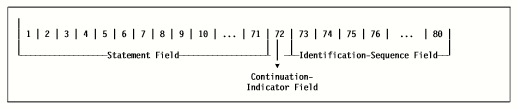
\includegraphics[width=\textwidth]{img/line}
	\caption{Description of line columns (source HLASM Language Reference https://www-01.ibm.com/servers/resourcelink/\-svc00100.nsf/\-pages/\-zOSV2R3sc264940/\-\$file/\-asmr1023.pdf).}
	\label{fig01:line}
\end{figure}


\section{Assembling}

Having briefly described syntax, this section prepares reader to better understand assembly process hidden behind HLASM. 

We can divide assembling into two interlinked steps, \textbf{conditional assembly} and \textbf{ordinary assembly}.

\subsection{Conditional assembly}

This part of assembly process can be compared to C++ text prepocessor. In HLASM it is more complicated process so it has obtained the term \textit{code generation}. It consists of \textbf{variable symbols}, \textbf{conditional assembly (CA) instructions} and \textbf{macros}. 


\subsubsection{Variable symbols}

These symbols serve as points of substitution or information holders. 

When they occur in a statement, they are substituted by their value to create a new statement. For example, in this manner user can write variable symbol in operation field of statement and generate any instruction that can be a result of substitution.

Variable symbols have also notion of types. Symbol can be integer, boolean or string. CA instructions gather this information for different sorts of conditional branching.

\subsubsection{CA instructions}

The major difference to other instructions is that they are not assembled into object code, they rather select which instructions will be processed by assembler next.

One subset of CA instructions operates on variable symbols. With them user can define variable symbols locally or globally, assign or update their value.

Other subset is capable of conditional and unconditional branching. HL\-ASM provides big variety of built in binary or unary operations on variable symbols which can create complex conditional expressions. This is important in HLASM as you can alter flow of instructions that will be assembled into executable program.

\subsubsection{Macros}
Macro is structure consisting of name, input parameters and sequence of statements called body. When they are called in HLASM program, each statement in the body is performed. Nested or recursive call of macros is allowed. Macro body can even contain such sequence of instructions that it can generate another macro definition ready for later use. With help of variable symbols, HLASM macros have power to create custom task specific macros.

\subsection{Ordinary assembly}

Ordinary assembly is a term for assembly other that conditional. 

Assembly of \textit{machine instructions} belong here. They and their operands are translated to sequence of bytes and written to executable program. HL\-ASM differs from basic assemblers as it allows expressions as operands of those instructions. This expressions can contain constanst as well as are capable of address arithmetics.

Assembly of \textit{assembler instructions} also belong here. However, they are neither assembled nor completely ignored. They alter behavior of assembler.

\subsubsection{Assembler instructions}
The behavior of assembler is altered by this instructions in different ways. Let us enumerate some of them.
 
\begin{itemize}
	\item \textbf{ICTL} --- Changes previously described line columns (i.e. \textit{begin column} at column 2 etc. ).
	
	\item \textbf{DC} --- Reserves space in object code for data described in operands field and assembles them in place (i.e. assembles float, double, character array, address etc. ).
	
	\item \textbf{EQU} --- Defines named constant with integer value or relative address value. This constants can be accessed by \textit{conditional assembly}, hence alter it in custom manner.
	
	\item \textbf{COPY} --- Copies whole file found in \textit{copy member library}\footnote{Path to library is passed to assembler before the start of assembly.} and pastes it in place of the instruction.
	
	\item \textbf{CSECT} --- Creates an executable control section. Serves as the beginning of a machine instruction sequence and start of relative addressing.
\end{itemize}

Here is example of simple HLASM program with the description of its statements.

\begin{verbatim}
         name        operation   operands
         
[01]                 MACRO                   
[02]     &NAME       GEN_LABEL
[03]     &NAME       EQU         *
[04]                 MEND
[05]             
[06]                 COPY        REGS
[07]             
[08]     TEST        CSECT
[09]     &VAR        SETA        L'DOUBLE
[10]                 AIF         (&VAR EQ 4).END
[11]     LBL1        GEN_LABEL
[12]                 LR          3,2
[13]                 L           8
[14]     LBL2        GEN_LABEL
[15]     LEN         EQU         LBL2-LBL1
[16]                 DC          (LEN)C'HELLO'
[17]     DOUBLE      DC          D'-3.729'
[18]     .END        ANOP
[19]                 END
\end{verbatim} 

In lines \verb|01-04| the reader can see \textit{macro definition}. It is defined with a name \verb|GEN_LABEL|, variable \verb|NAME| and has one instruction in body that assigns to label in \verb|NAME| current address.

In line \verb|06| there is use of \textit{copy instruction} where it includes contents of \verb|REGS| file.

Line \verb|08| establishes start of executable section called \verb|TEST|. 

In line \verb|09| integer value is assigned to variable symbol \verb|VAR|. The value is the length attribute of non previously defined constant \verb|DOUBLE|. The assembler looks for definition of the constant to properly evaluate conditional assembly expression. In the next line there is CA branching instruction \verb|AIF|. If value of \verb|VAR| equals 4, next lines are skipped and assembling continues on line \verb|18| where branching symbol \verb|END| is located.  

Lines \verb|12-13| shows example of machine instructions which are directly assembled into object code. Lines \verb|11,14| are examples of macro call.

In line \verb|15| to constant \verb|LEN| is equated difference of two addresses. This value is next used to generate character data.

Instruction \verb|DC| in line \verb|17| creates value of type double and assigns its address to constant \verb|DOUBLE|. This constant also holds information about length, type and other attributes of the data.  

\verb|ANOP| is empty assembler action and line \verb|19| ends the program assembling. 

\vspace{5mm}
As the reader may see, HLASM is heavily extended assembler with complex assembling phases. 
However, the result of that is programming language with large expressive power. 
